% This paper is part of the single transits project.
% Copyright 2015 Dan Foreman-Mackey (NYU) and the co-authors listed below.
%
%  RULES OF THE GAME
%
%  * 80 characters
%  * line breaks at the ends of sentences
%  * eqnarrys ONLY
%  * ``light curve'' not ``light-curve'' or ``lightcurve''
%  * that is all.
%

% \documentclass[twocolumn]{aastex6}
\documentclass[onecolumn]{aastex6}
% \documentclass[preprint]{aastex}

\pdfoutput=1

\usepackage{color,hyperref}
\definecolor{linkcolor}{rgb}{0,0,0.5}
\hypersetup{colorlinks=true,linkcolor=linkcolor,citecolor=linkcolor,
            filecolor=linkcolor,urlcolor=linkcolor}
\usepackage{url}
\usepackage{amssymb,amsmath}
\usepackage{subfigure}
\usepackage{booktabs}

\usepackage{natbib}
\bibliographystyle{aasjournal}

\newcommand{\project}[1]{\textsl{#1}}
\newcommand{\kepler}{\project{Kepler}}
\newcommand{\KT}{\project{K2}}
\newcommand{\tess}{\project{TESS}}
\newcommand{\plato}{\project{PLATO}}
\newcommand{\jwst}{\project{JWST}}
\newcommand{\terra}{\project{TERRA}}
\newcommand{\pdc}{\project{PDC}}
\newcommand{\license}{MIT License}

\newcommand{\paper}{article}

\newcommand{\foreign}[1]{\emph{#1}}
\newcommand{\etal}{\foreign{et\,al.}}
\newcommand{\etc}{\foreign{etc.}}
\newcommand{\True}{\foreign{True}}
\newcommand{\Truth}{\foreign{Truth}}

% \newcommand{\figref}[1]{\ref{fig:#1}}
% \newcommand{\Fig}[1]{\figurename~\figref{#1}}
% \newcommand{\fig}[1]{\Fig{#1}}
\newcommand{\figlabel}[1]{\label{fig:#1}}

% \newcommand{\Tab}[1]{Table~\ref{tab:#1}}
% \newcommand{\tab}[1]{\Tab{#1}}
\newcommand{\tablabel}[1]{\label{tab:#1}}

\renewcommand{\eqref}[1]{\ref{eq:#1}}
\newcommand{\Eq}[1]{Equation~(\eqref{#1})}
\newcommand{\eq}[1]{\Eq{#1}}
\newcommand{\eqalt}[1]{Equation~\eqref{#1}}
\newcommand{\eqlabel}[1]{\label{eq:#1}}

\newcommand{\sectionname}{Section}
\newcommand{\sectref}[1]{\ref{sect:#1}}
\newcommand{\Sect}[1]{\sectionname~\sectref{#1}}
\newcommand{\sect}[1]{\Sect{#1}}
\newcommand{\sectalt}[1]{\sectref{#1}}
\newcommand{\App}[1]{Appendix~\sectref{#1}}
\newcommand{\app}[1]{\App{#1}}
\newcommand{\sectlabel}[1]{\label{sect:#1}}

\newcommand{\T}{\ensuremath{\mathrm{T}}}
\newcommand{\dd}{\ensuremath{\,\mathrm{d}}}
\newcommand{\unit}[1]{{\ensuremath{\,\mathrm{#1}}}}
\newcommand{\bvec}[1]{{\ensuremath{\boldsymbol{#1}}}}
\newcommand{\appropto}{\mathrel{\vcenter{
  \offinterlineskip\halign{\hfil$##$\cr
    \propto\cr\noalign{\kern2pt}\sim\cr\noalign{\kern-2pt}}}}}
\newcommand{\densityunit}{{\ensuremath{\mathrm{nat}^{-2}}}}

% TO DOS
\newcommand{\todo}[3]{{\color{#2}\emph{#1}: #3}}
\newcommand{\dfmtodo}[1]{\todo{DFM}{red}{#1}}
\newcommand{\hoggtodo}[1]{\todo{HOGG}{blue}{#1}}

% Notation for this paper.
\newcommand{\meanpars}{{\ensuremath{\bvec{\theta}}}}
\newcommand{\kernpars}{{\ensuremath{\bvec{\alpha}}}}

\newcommand{\params}{{\ensuremath{\bvec{w}}}}
\newcommand{\poppars}{{\ensuremath{\bvec{\beta}}}}


\newcommand{\datareleaseurl}{{\url{http://bbq.dfm.io/ketu}}}

% no more bad lines!
\sloppy\sloppypar

% \slugcomment{Not to appear in Nonlearned J., 45.}

\begin{document}

\title{%
The population of long-period exoplanets I. --- \\
Fully-automated discovery \& characterization of
long-period transiting exoplanet candidates in the \kepler\ archive
}

\newcounter{affilcounter}
\setcounter{affilcounter}{2}
\altaffiltext{1}{\url{danfm@uw.edu}; Sagan Fellow}

\edef \uw {\arabic{affilcounter}}\stepcounter{affilcounter}
\altaffiltext{\uw}       {Astronomy Department, University of Washington,
                          Seattle, WA, 98195, USA}

\edef \scda {\arabic{affilcounter}}\stepcounter{affilcounter}
\altaffiltext{\scda}     {Simons Center for Data Analysis, 160 Fifth Avenue,
                          7th floor, New York, NY 10010, USA}

\edef \nyu       {\arabic{affilcounter}}\stepcounter{affilcounter}
\altaffiltext{\nyu}      {Center for Cosmology and Particle Physics,
                          New York University,
                          4 Washington Place, New York, NY, 10003, USA}

\edef \cds       {\arabic{affilcounter}}\stepcounter{affilcounter}
\altaffiltext{\cds}      {Center for Data Science, New York University,
                          726 Broadway, 7th Floor, New York, NY, 10003, USA}

\edef \mpia      {\arabic{affilcounter}}\stepcounter{affilcounter}
\altaffiltext{\mpia}     {Max-Planck-Institut f\"ur Astronomie,
                          K\"onigstuhl 17, D-69117 Heidelberg, Germany}

\edef \princeton {\arabic{affilcounter}}\stepcounter{affilcounter}
\altaffiltext{\princeton}{Department of Astrophysics, Princeton University,
                          Princeton, NJ, 08544, USA}

\edef \mpis      {\arabic{affilcounter}}\stepcounter{affilcounter}
\altaffiltext{\mpis}     {Max Planck Institute for Intelligent Systems
                          Spemannstrasse 38, 72076 T\"ubingen, Germany}

\author{%
    Daniel~Foreman-Mackey\altaffilmark{1,\uw},
    David~W.~Hogg\altaffilmark{\scda,\nyu,\mpia,\cds},
    Timothy~D.~Morton\altaffilmark{\princeton},
    Bernhard~Sch\"olkopf\altaffilmark{\mpis},
    Eric~Agol\altaffilmark{\uw},
    and others
}



\begin{abstract}

The \kepler\ Mission has discovered thousands of exoplanets and revolutionized
our understanding of their population.
This large, homogeneous catalog of discoveries has enabled rigorous studies of
the occurrence rate of exoplanets and extra-Solar planetary systems as a
function of their physical properties.
Transit survey like \kepler\ are most sensitive to planets with shorter
orbital periods than the gas giant planets that dominate the dynamics of our
Solar System.
We performed a fully-automated search for the transits of long-period
exoplanets in the archival \kepler\ light curves and announce XXX planet
candidates.
Since our method involves no human intervention, we empirically characterize
the completeness and reliability of our search.
Based on these results, we measure the average occurrence rate of exoplanets
smaller than Jupiter and with orbital periods longer than 700 days to be $\dd
N = YYY \pm ZZZ\dd \ln P \dd \ln R$.

\end{abstract}

\keywords{%
methods: data analysis
---
methods: statistical
---
catalogs
---
planetary systems
---
stars: statistics
}

\section{Introduction}

The transit method of exoplanet detection and characterization has been
demonstrated as a powerful method for building systematic catalogs of
exoplanets.
Despite the great success of the \kepler\ Mission with thousands of planet
discoveries \citep{Burke:2014, Rowe:2015}, current methods for exoplanet
discoveries are currently limited in the range of orbital periods that can be
studied.
Specifically, the standard transit search procedures only discover signals
with at least three observed transits \citep[for example][]{Petigura:2013,
Burke:2014, Rowe:2015}.
For \kepler, with a baseline of about four years, this sets an absolute upper
limit on the detectable periods of about two years.
In the Solar System, Jupiter---with a period of 12 years---dominates the
planetary dynamics and, since it would only exhibit at most one transit in the
\kepler\ data, it would be missed by most existing transit search procedures.
It is possible to discover long-period planets like this using targeted radial
velocity (RV) surveys \citep[for example][]{Butler:2006, Knutson:2014}
\dfmtodo{CITE Bryan \etal} but the cost of implementing a systematic RV search
is substantially higher than searching the existing and forthcoming
photometric data for single transits.

There are two main technical barriers to a search for single transit events.
The first is that the transit probability for long-period planets is very low;
scaling as $\propto P^{-5/3}$ for orbital periods longer than the
baseline of contiguous observations.
Therefore, even if long-period planets are intrinsically common, they will
still be underrepresented in a transiting sample.
The second challenge is that there are substantial signals in the observed
light curves caused by stochastic processes---both instrumental
(pointing jitter, temperature variations, \etc) and astrophysical (stellar
variability, \etc)---that can masquerade as transit signals.
In practice, even using the most sophisticated systematics removal methods,
these false signal far outnumber the true single transits.

Nearly every transit search algorithm is built on the same principles and many
of the same decisions are made.
In particular, at the heart of most methods is a matched filtering step where
the likelihood of an approximate transit model is computed on a grid in the
physical parameters \citep[\kepler\ Data Processing
Handbook\footnote{\url{https://archive.stsci.edu/kepler/manuals/KSCI-19081-001_Data_Processing_Handbook.pdf}};][]{%
Petigura:2013, Huang:2013, Dressing:2015, Foreman-Mackey:2015}.
Using these methods, and substantial hand-curation, some long-period
transiting candidates have been published \citep[for example][]{Batalha:2013,
Huang:2013, Kipping:2014a}.
For more recent data releases, the community has settled on more conservative
selection criteria where candidates are required to have multiple transits
\citep[for example][]{Petigura:2013, Burke:2014, Rowe:2015}.
Even the \project{QATS} algorithm \citep{Carter:2013} for finding
quasiperiodic transits builds on much the same infrastructure.
This means that there has never been a systematic search for single transits
in the full \kepler\ dataset.

A qualitatively different approach to planet search is employed by the
\project{Planet Hunters} (PH)
project\footnote{\url{http://www.planethunters.org/}} \citep{Fischer:2012}.
PH is a ``citizen science'' project where visitors to the website look at
sections of light curve and mark the locations of transits that can be
identified visually.
Visual inspection can be a useful search technique for large single transits
because humans are able to robustly distinguish transit signals from the noise
and this project has yielded some promising long-period candidates and
confirmed planets \citep[for example][]{Wang:2013} \dfmtodo{CITE Wang 2015}.
One shortcoming of the PH method is that it can be difficult to fully quantify
the performance (completeness and reliability) of the search and PH does not
evaluate their users using synthetic transit signals as is now common practice
in the transit search literature \dfmtodo{is this still true?}.
This means that the PH sample of candidates cannot be used for robust
population inference.

To study the occurrence rate of long-period exoplanets, we have developed a
fully-automated method for searching the archival \kepler\ light curves for
these systems with only one or two transits.
Using this method, we detect XXX long-period transiting planet candidates and
YYY long-period eclipsing binary candidates.
We estimate that the population level false positive rate in this exoplanet
candidate sample is about ZZZ\%.
By injecting synthetic transit signals into the \kepler\ light curves, we
measure the completeness of our search method.
Based on this catalog of exoplanet candidates and the search completeness, we
constrain the occurrence rate of long-period exoplanets.
For large planets, these results are consistent with previous measurements of
long-period, giant planet occurrence rates based on radial velocity surveys
and we demonstrate that small---and possibly rocky---planets are more common
than their larger counterparts even at long orbital periods.

Data from the \kepler\ Mission has been used to discover a diverse zoo of
thousands of exoplanets of all sizes orbiting stars of all types.
It has be demonstrated that these catalogs of exoplanet discoveries can be
used to place constraints on the occurrence rate of exoplanets \dfmtodo{CITE}.
These results are sensitive to the detection efficiency and reliability of the
discovery methodology \dfmtodo{CITE Burke}.

\section{A fully-automated search method}

To find long-period exoplanets in the \kepler\ light curves, we search for
individual, high signal-to-noise transit signals using a fully-automated
procedure that can be broken into three main steps:
\begin{enumerate}
{\item an initial candidate search using a box-shaped matched filter,}
{\item light curve-level vetting (using automated model comparison) to remove
signals that don't match a transit shape, and}
{\item pixel-level vetting to remove some astrophysical false positives.}
\end{enumerate}
The following sections describe each of these steps in more detail.

\subsection{Finding box-shaped candidate events}

It is not feasible to compute a full model comparison at every time in the
light curve so we must first find potentially interesting events.
To generate this list, we apply a standard ``box least squares'' (BLS;
\dfmtodo{CITE}) method with a single (non-periodic) box.
First, we filter the PDC (\dfmtodo{CITE}) light curves using a running
windowed median with a half-width of \dfmtodo{how many} to remove stellar
variability.
We then compute the signal-to-noise of the depth of a 0.6~day long transit on
a grid of times spanning the full \kepler\ baseline.
To avoid edge effects, we apodize this detection scalar near any large gaps in
the time series using a logistic function with width equal to one transit
duration.
Finally, we estimate the noise in the time series using a robust running
windowed variance estimate of the detection scalar and accepting peaks more
than 25-times this noise as candidates.

\subsection{Light curve-level vetting}

In this step of the method, the goal is to discard any signals that are not
sufficiently ``transit-like'' in shape.
To quantify this decision, we perform a model comparison between a physical
transit model and a set of other parameterized models for systematics.
In order for a candidate to pass this vetting step, the transit model must be
``preferred'' to any other model as measured using the Bayesian Information
Criterion (BIC).
The BIC is not the optimal choice for this model comparison but it is
computationally intractable to compute thousands of precise marginalized
likelihoods for each model.
The BIC can be efficiently computed and it exhibits the desired
behavior---increasing with the likelihood but flexible models are
penalized---and we find that it performs sufficiently well in practice.

For up to three candidate transit times per light curve, we select a
contiguous chunk of PDC light curve approximately centered on the proposed
transit with no more than 500 cadences \dfmtodo{check me} and compute the BIC
of each model for this data set.
We will define the BIC for a model $k$ in the set of $K$ models is given by
\begin{eqnarray}
\mathrm{BIC}_k &=& \ln \mathcal{L}^* - \frac{J}{2}\,\log N
\end{eqnarray}
where the likelihood function $\mathcal{L}$ is evaluated at its maximum, $J$
is the number of free parameters in the model, and $N$ is the number of
data points in the data set.

For each model, we describe the data using a Gaussian Process (GP;
\dfmtodo{cite}) with a Mat\'ern-3/2 covariance and mean given by the chosen
model $m_k(t;\,\meanpars)$ parameterized by the parameter vector \meanpars.
This generative model is specified by the following likelihood function:
\begin{eqnarray}
\mathcal{L} = \ln p_k(\bvec{y}\,|\,\meanpars,\,\kernpars) &=&
- \frac{1}{2}\,\bvec{r}_k(\meanpars)^\T\,K(\kernpars)^{-1}\,
    \bvec{r}_k(\meanpars)
- \frac{1}{2}\log\det K(\kernpars) - \frac{N}{2} \log{2\,\pi}
\end{eqnarray}
where \bvec{y} is the vector of flux measurements, \bvec{t} are the
corresponding times, and
\begin{eqnarray}
\bvec{r}_k(\meanpars) &=& \bvec{y} - m_k(\bvec{t};\,\meanpars) \quad.
\end{eqnarray}
The covariance matrix $K(\kernpars)$ is parameterized by the parameters
$\kernpars = (\alpha,\,\tau)$ and its elements are given by
\begin{eqnarray}
\left[ K(\kernpars) \right]_{ij} &=& \sigma_i^2\,\delta_{ij}
    + \alpha^2 \left[ 1+\frac{|t_i - t_j|}{\sqrt{3}\,\tau} \right]
      \exp \left(-\frac{|t_i - t_j|}{\sqrt{3}\,\tau}\right)
\end{eqnarray}
where $\sigma_i$ is the reported uncertainty on the $i$-th flux measurement.

The gradients of the likelihood with respect to the parameters \meanpars\
and \kernpars\ are given by
\begin{eqnarray}
\frac{\dd\ln p_k(\bvec{y}\,|\,\meanpars,\,\kernpars)}{\dd \meanpars} &=&
\frac{\dd m_k(\bvec{t};\,\meanpars)}{\dd\meanpars}^\T \, K(\kernpars)^{-1} \,
    m_k(\bvec{t};\,\meanpars)
\end{eqnarray}
and
\begin{eqnarray}
\frac{\dd\ln p_k(\bvec{y}\,|\,\meanpars,\,\kernpars)}{\dd \kernpars} &=&
\frac{1}{2}\,\mathrm{Tr}\left(
    \left[ \bvec{\phi}\,\bvec{\phi}^\T - K(\kernpars)^{-1} \right]
    \,\frac{\dd K(\kernpars)}{\dd\kernpars}
\right)
\end{eqnarray}
where
\begin{eqnarray}
\bvec{\phi} &=& K(\kernpars)^{-1}\,\bvec{r}_k(\meanpars) \quad.
\end{eqnarray}
Therefore, if we can compute the gradient of the model with respect to its
parameters, we can efficiently optimize this function to find the maximum
likelihood parameters using a gradient-based non-linear optimization method.
To compute the gradients of the transit model, we use a compile-time automatic
differentiation library \dfmtodo{cite Ceres} and for the other models, we
choose models that can be easily differentiated analytically.

The models are:
\begin{itemize}
{\item a limb-darkened, exposure time integrated transit light curve,}
{\item a pure Gaussian Process model to capture stellar variability,}
{\item a single outlier,}
{\item an step function, and}
{\item a box.}
\end{itemize}


\subsection{Pixel-level vetting}


\begin{figure*}
\begin{center}
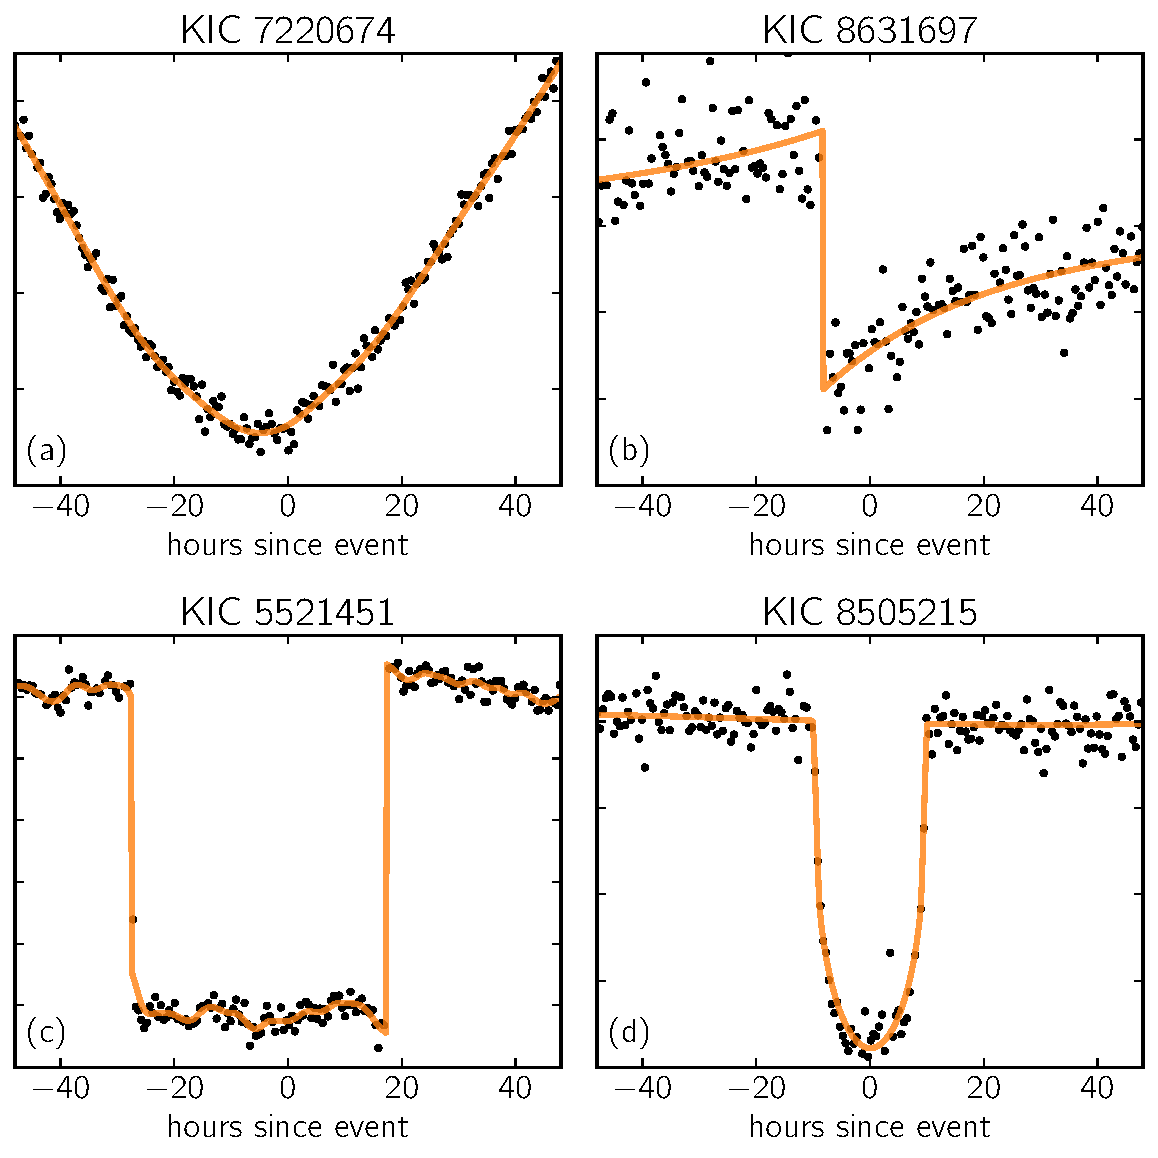
\includegraphics[width=\textwidth]{figures/model_comp.pdf}
\end{center}
\caption{%
Representative examples of candidate events flagged by the initial search.
Each example falls into a different model category and the figure shows the
data as black points and the best fit mean model prediction.
The examples represent the following model categories:
\emph{(a)} variability, \emph{(b)} step, \emph{(c)} box, and \emph{(d)}
transit.
\figlabel{model-comp}}
\end{figure*}


\section{A catalog of exoplanet \& binary candidates}


\subsection{Target selection}\sectlabel{data}

For the purposes of this \paper, we select the $\sim40,000$ brightest and
quietest G and K dwarfs from the \kepler\ catalog using the following
parameters:
\begin{itemize}
{\item $4200\unit{K} \le T_\mathrm{eff} \le 6100\unit{K}$,}
{\item $R_\star \le 1.15\,R_\odot$,}
{\item $K_p \le 15\unit{mag}$, and}
{\item $\mathrm{CDPP}_{7.5\unit{hrs}} \le 1000\unit{ppm}$.}
\end{itemize}
We also restrict the sample to only include targets with a data span of more
than two years and a duty cycle of better than $0.6$.
Since the \kepler\ data have been searched for shorter period planets
\dfmtodo{CITE Coughlin} and eclipsing binaries \dfmtodo{CITE EB catalog} than
targeted by this project, we censor these previously known targets.
For the known EBs, we simply remove these targets from the candidate list.
For the confirmed and candidate KOIs from \dfmtodo{Coughlin}, we remove data
within 2 transit durations of the known candidates.

\begin{figure*}
\begin{center}
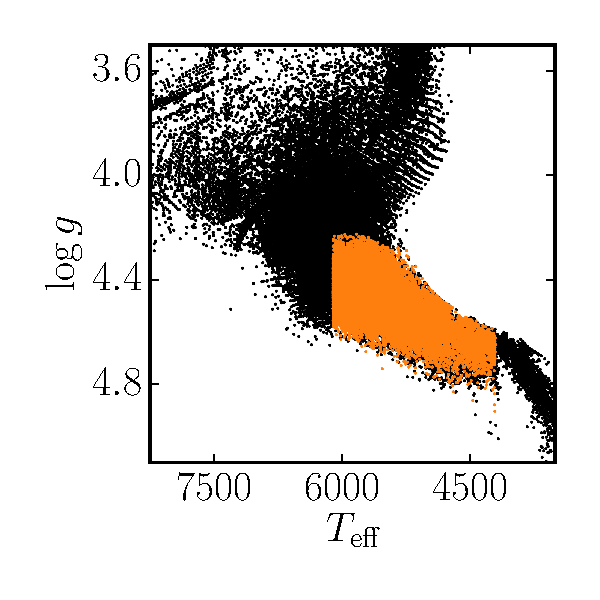
\includegraphics{figures/targets.pdf}
\end{center}
\caption{%
Blah.
\figlabel{targets}}
\end{figure*}


We start with the PDC-MAP light curves downloaded from
MAST\footnote{\url{https://archive.stsci.edu/kepler/}}.



The \kepler\ Mission measured photometric time series for about 190,000 stars
at half-hour cadence for a baseline of over four years.
We aim to search these light curves for single transits of long-period planets
and single eclipses of binary stars.
These data are made available on
MAST\footnote{\url{https://archive.stsci.edu/kepler/}} and, for each target,
we downloaded the full set of long cadence light curve files provided by Data
Release 24 \citep{Thompson:2015}.
From these files, we extracted the PDC time series and split them into
``sections'' with no more than ten contiguous missing or flagged data points.
The PDC light curves have been corrected for the instrumental effects caused
by the spacecraft using a data-driven model of the focal plane
\citep{Stumpe:2012, Smith:2012}.
Crucially, an attempt is also made by the PDC procedure to remove sharp
instrumental artifacts like ``sudden pixel sensitivity dropouts (SPSDs)''.
The success rate of this correction procedure is much higher than in earlier
data releases but, as discussed in \sect{demo}, there remain some cases that
are not properly accounted for.

The goal of this project is to discover the transits of long-period planets
that have not yet been discovered.
Therefore, when studying the light curve of an eclipsing binary star or a star
with known transiting planet candidates---on shorter periods---we also remove
all the in-transit data for the candidate using the parameters provided by the
\project{NASA Exoplanet
Archive}\footnote{\url{http://exoplanetarchive.ipac.caltech.edu/}; We
downloaded the \texttt{cumulative} table of \kepler\ Objects of Interest on
2015-03-25.}.


\subsection{Parameter estimation}


\begin{figure*}
\begin{center}
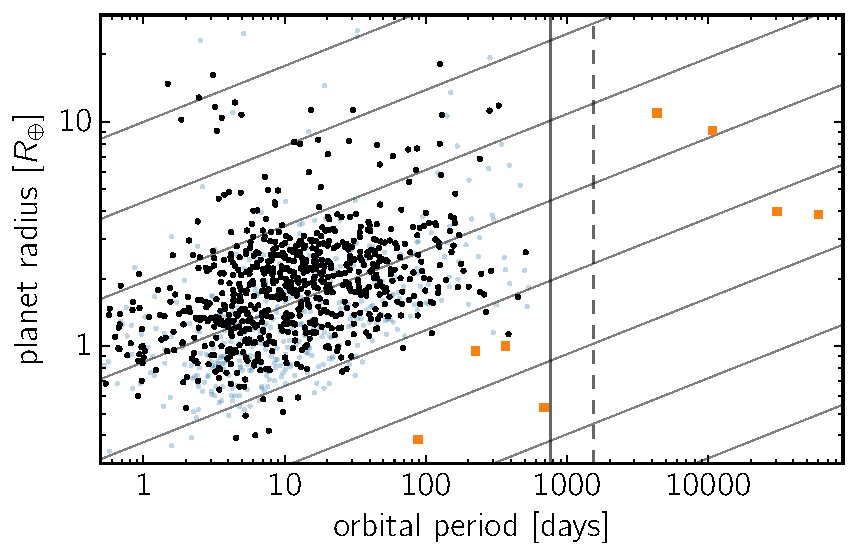
\includegraphics{figures/full_sample.pdf}
\end{center}
\caption{%
Blah.
\figlabel{full-sample}}
\end{figure*}


\subsection{Discussion of some interesting systems}



\section{Empirical search completeness}

To measure the completeness of our long-period transit search method, we
exploit the fact that transit signals are sparse and rare.
Therefore, most light curves contain no transits and we can reliably measure
the recovery rate of our method on synthetic transit signals---with known
properties---injected into real light curves.
This procedure is standard practice in the transit literature and it has been
used to determine the completeness of the KOI catalog (\dfmtodo{cite}) and
other independent transit searches (\dfmtodo{cite}).

To reliably capture the full structure of the search completeness function,
the simulations must sample the (high-dimensional) space of all properties
that affect the probability of detecting a transit: the stellar properties
(including variability amplitudes and time scales), the planet's physical
properties and orbital elements, and any observational effects (noise,
spacecraft pointing variations, \etc).
For the modest goals of this paper, we only need a robust constraint on the
transit detection efficiency \emph{integrated} across the target sample but,
even so, many simulations per star are required.

The procedure for measuring the recovery rate of simulated transits is as
follows:
\begin{enumerate}
{\item First, a star is randomly selected from the target list, and the PDC
light curve and stellar properties for that star are loaded.}
{\item Planetary properties are sampled from the distributions listed in
\dfmtodo{some table} with phase uniformly distributed across the baseline of
observations. These properties are resampled until the transit is visible in
at least one non-flagged cadence.}
{\item The transit signal induced by this planet is computed and multiplied
into the PDC light curve.}
{\item The transit search method described in section \dfmtodo{some section}
(including de-trending and all automated vetting) is applied to this light
curve with the injected transit signal.}
{\item This candidate is flagged as recovered if at least one transit (within
\dfmtodo{some tolerance}) passes all the cuts imposed by the automated
vetting.}
\end{enumerate}

The fraction of recovered simulations as a function of the relevant parameters
gives an estimate of the search completeness or the probability of detecting
an exoplanet transit with a given set of parameters, \emph{conditioned on the
fact that it transits}.
We will call this function $Q_{\mathrm{det},k}(\params)$ where \params\ is the
set of all parameters affecting the transit detectability and $k$ is an index
running over target stars.

This detection efficiency must then be combined with the geometric transit
probability function and the window function.
For the star $k$, the geometric transit probability is given by \dfmtodo{cite}
\begin{eqnarray}
Q_{\mathrm{geom},k} (\params) &=& \frac{R_{\star,k}}{a_k}
    \, \frac{1 + e\,\sin\omega}{1-e^2} \\
&=& \left[\frac{4\,\pi^2}{G\,M_{\star,k}}\right]^{1/3}\,R_{\star,k}
    \, \left[\frac{1 + e\,\sin \omega}{1-e^2}\right]
    \, P^{-2/3}
\end{eqnarray}
where the parameters $e$, $\omega$, and $P$ are included in \params.
Approximating the window function using the binomial probability of observing
at least one transit \dfmtodo{cite bm14} we find
\begin{eqnarray}
Q_{\mathrm{win},k} (\params) &=& 1 - (1 - f_{\mathrm{duty},k})^{T_k/P}
\end{eqnarray}
where $f_{\mathrm{duty},k}$ is the duty cycle and $T_k$ is the full
observation baseline for target $k$.

Combining these detection effects, the total detection efficiency is given by
\begin{eqnarray}
Q_k(\params) &=& Q_{\mathrm{det},k}(\params) \,
                 Q_{\mathrm{win},k} (\params) \,
                 Q_{\mathrm{geom},k} (\params) \quad.
\end{eqnarray}
For the purposes of this \paper, we are not considering the occurrence rate of
exoplanets as a function of stellar properties; we will only measure an
average rate across the target sample that we previously selected.
Therefore, it is sufficient to estimate the marginalized detection efficiency
integrated with respect to our prior distributions on the nuisance parameters.
In this case, the only parameters that we will consider are planet radius and
orbital period.
Under this model, the relevant detection efficiency function for long-period
transiting planets is
\begin{eqnarray}\eqlabel{full-comp}
Q(R,\,P) &=& \frac{1}{K} \sum_{k=1}^{K} \int Q_k(\params) \,
    p(\params_{\{R,\,P\}}) \dd\params_{\{R,\,P\}}
\end{eqnarray}
where $\params_{\{R,\,P\}}$ indicates the set of all parameters except radius
and period.

Since the simulated parameters in the injection and recovery tests described
above were sampled from the prior distribution $p(\params_{\{R,\,P\}})$, the
easiest way to estimate \eq{full-comp} is to take the ratio of the weighted
histogram of the recovered injections to the weighted histogram of all
simulations where each simulation is weighted by
$Q_{\mathrm{win},k} (\params) \, Q_{\mathrm{geom},k} (\params)$ evaluated at
the parameters of the simulation.


\section{The occurrence rate of long-period exoplanets}

Geometric:

Temporal:

\begin{eqnarray}
Q_{\mathrm{temp},k} (\params) &=& \frac{T_k}{P}
\end{eqnarray}
where $T_k$ is the total observing baseline for target $k$.
Combined with the detection efficiency $Q_{\mathrm{det}}(\params)$ (assumed to
be constant for each target), the total completeness as a function of the
parameters is
\begin{eqnarray}
Q_k(\params) &=& Q_{\mathrm{det},k}(\params) \,
                 Q_{\mathrm{temp},k} (\params) \,
                 Q_{\mathrm{geom},k} (\params) \\
&=& Q_{\mathrm{det},k}(\params) \,
    \left[\frac{4\,\pi^2}{G\,M_{\star,k}}\right]^{1/3}\,
    R_{\star,k}\,T_k
    \, \left[\frac{1 + e(\params)\,\sin \omega(\params)}{1-e(\params)^2}\right]
    \, P^{-5/3} \quad.
\end{eqnarray}

The likelihood function for the catalog of planet candidates is
\begin{eqnarray}
p(\{\params_n\}\,|\,\poppars) &\propto&
    \exp \left(
        \int f_\poppars (\params)\,\sum_{k=1}^K Q_k(\params) \dd\params
    \right) \, \prod_{n=1}^N f_\poppars (\params_n) \quad.
\end{eqnarray}

Therefore
\begin{eqnarray}
\int f_\poppars (\params)\,\sum_{k=1}^K Q_k(\params) \dd\ln P\dd\ln R &=&
    \bar{Q}\,\int Q_{\mathrm{det}}(\params)\,f_\poppars(\params)\,P^{-5/3}
        \dd\ln P\dd\ln R
\end{eqnarray}
where
\begin{eqnarray}
\bar{Q} &=& \sum_{k=1}^K
    \left[\frac{4\,\pi^2}{G\,M_{\star,k}}\right]^{1/3}\,R_{\star,k}\,T_k
\quad.
\end{eqnarray}

The easiest way to evaluate this integral in practice is to use Monte Carlo
integration to find
\begin{eqnarray}
\int Q_{\mathrm{det}}(\params)\,f_\poppars(\params)\,P^{-5/3}\dd\ln P\dd\ln R
&=& \frac{F}{J}\sum_{j=1}^J Q_{\mathrm{det}}(P^{(j)},\,R^{(j)})\,
        f_\poppars(P^{(j)},\,R^{(j)})
\end{eqnarray}
where
\begin{eqnarray}
F &=& \frac{3}{5}\,[P_\mathrm{min}^{-5/3}-P_\mathrm{max}^{-5/3}]\,
      [\ln R_\mathrm{max} - \ln R_\mathrm{min}]
\end{eqnarray}
and
\begin{eqnarray}
P^{(j)} \sim P^{-8/3} &\mathrm{and}&
\ln R^{(j)} \sim \mathcal{U}(\ln R_\mathrm{min},\,\ln R_\mathrm{max})
\end{eqnarray}


\begin{eqnarray}
f_\poppars (\params) &=& \frac{1}{f_0}\,C\,P^\alpha\,R^\beta
\end{eqnarray}
where
\begin{eqnarray}
f_0 &=&
    \int_{P_\mathrm{min}}^{P_\mathrm{max}}
    \int_{R_\mathrm{min}}^{R_\mathrm{max}}
    P^\alpha\,R^\beta\dd\ln P\dd\ln R
\end{eqnarray}


\section{Astrophysical false positives}

Tim to write some words here.



\section{Discussion}\sectlabel{discussion}

The discovery and characterization of transiting planets based on a single
transit event is crucial for the future of transiting exoplanet surveys.
Many of the most dynamically influential planets---like Jupiter in our Solar
system---exhibit only a single transit in the full observational baseline of
the \kepler.
This will become even more of a problem as upcoming surveys move to shorter
contiguous observations.
For example, the \tess\ Mission is planned to get full-sky coverage at
half-hour cadence but most of the sky will only be targeted for a month.
This means that even habitable zone planets orbiting cool stars will transit
their host \emph{at most once in the entire lifetime of the Mission}!

To date, no methods exist for systematically and robustly discovering single
transit events based on large photometric surveys.
In this \paper, we present a novel and conceptually unique solution to this
problem drawing on machine learning methods for supervised classification.
This method has immense potential because it can be designed to be very robust
to false positives and it can exploit the detailed shape of physical transits.

Despite the fact that single transits are unlikely even if these long-period
planets are intrinsically common, we estimate that $\sim 60$ events should be
detectable in the \kepler\ archival dataset by extrapolating recent models of
planet occurrence rates and taking selection effects into account.
When applied to 3500 light curves from the \kepler\ dataset, this method
recovers one previously unknown single transit event at
$830.8093\pm0.0002$~KBJD in the light curve of KIC 10602068.
This rate is consistent with the predicted yield of 60 events in the full
dataset of 190,000 light curves.

Assuming a bound Keplerian orbit, we place constraints on the physical
properties of this transit candidate KIC 10602068.01.
Using photometrically derived stellar properties, we find that this candidate
has a radius of $2.1 \pm 0.4\,R_\mathrm{J}$ placing it as a very large planet
or brown dwarf or a small star.

This method for transit search is built using supervised classification and
its performance relies on several strong assumptions about the datasets and
these assumptions are sometimes violated leading to some transit-like signals
that appear to be caused by noise to be misclassified as transits.
The most severe assumption is that the noise properties of the data are
stationary.
In other words, we assume that variability in one subset of a light curve is
completely spanned by the variability in the other sections.
This assumption is, in general, false because the stochastic processes that
cause stellar variability are complicated and non-stationary and the detector
is plagued by non-negligible catastrophic changes in sensitivity and response.
We attempt to mitigate this problem by using light curves that have been
preprocessed to remove most of the instrumental effects and carefully dividing
the data into subsets but some false positives are still incorrectly
identified as candidates.

One possible method for reducing the false positive rate would be to augment
the training dataset using heuristic simulations of common false positives or
the light curves of ``similar'' stars.
Another option is to recognize that this search drastically reduces the
parameter space requiring evaluation and comparing the predictive power of
a transit model to other heuristic models including stellar variability or
instrumental effects.


\acknowledgments
It is a pleasure to thank
\ldots
for helpful contributions to the ideas and code presented here.
DFM and DWH were partially supported by the National Science Foundation
(grant IIS-1124794),
the National Aeronautics and Space Administration
(grant NNX12AI50G), and the Moore--Sloan Data Science Environment at NYU.

This research made use of the NASA \project{Astrophysics Data System} and the
NASA Exoplanet Archive.
The Archive is operated by the California Institute of Technology, under
contract with NASA under the Exoplanet Exploration Program.
This \paper\ includes data collected by the \kepler\ mission. Funding for the
\kepler\ mission is provided by the NASA Science Mission directorate.
We are grateful to the entire \kepler\ team, past and present.
Their tireless efforts were all essential to the tremendous success of the mission
and the successes of \KT, present and future.
These data were obtained from the Mikulski Archive for Space Telescopes
(MAST).
STScI is operated by the Association of Universities for Research in
Astronomy, Inc., under NASA contract NAS5-26555.
Support for MAST is provided by the NASA Office of Space Science via grant
NNX13AC07G and by other grants and contracts.
Computing resources were provided by High Performance Computing (HPC) at New
York University (NYU).

\facility{Kepler}

\appendix

\section{Supervised classification}


\clearpage
\bibliography{peerless}
\clearpage


% \begin{figure}[p]
% \begin{center}
% \includegraphics{figures/pca.pdf}
% \end{center}
% \caption{%
% The top 10 eigen light curves (ELCs) generated by running principal component
% analysis on all the aperture photometry from Campaign~1.
% \figlabel{pca}}
% \end{figure}

\end{document}
